\documentclass[notes,11pt, aspectratio=169]{beamer}

\usepackage{pgfpages}
\setbeameroption{hide notes} % Only slide

\usepackage{array}
\usepackage{tikz}
\usepackage{verbatim}
\setbeamertemplate{note page}{\pagecolor{gray!5}\insertnote}
\usetikzlibrary{positioning}
\usetikzlibrary{snakes}
\usetikzlibrary{calc}
\usetikzlibrary{arrows}
\usetikzlibrary{decorations.markings}
\usetikzlibrary{shapes.misc}
\usetikzlibrary{matrix,shapes,arrows,fit,tikzmark}
\usepackage{amsmath}
\usepackage{mathpazo}
\usepackage{hyperref}
\usepackage{lipsum}
\usepackage{multimedia}
\usepackage{graphicx}
\usepackage{multirow}
\usepackage{dcolumn}
\usepackage{bbm}
\newcolumntype{d}[0]{D{.}{.}{5}}

\usepackage{changepage}
\usepackage{appendixnumberbeamer}

\usepackage[space]{grffile}
\usepackage{booktabs}

% Colors
\definecolor{blue}{RGB}{0,114,178}
\definecolor{red}{RGB}{213,94,0}
\definecolor{yellow}{RGB}{240,228,66}
\definecolor{green}{RGB}{0,158,115}
\definecolor{solutionbg}{RGB}{240,248,240}
\definecolor{solutionframe}{RGB}{0,158,115}

% Solution box environment for worked answers
\usepackage{tcolorbox}
\newtcolorbox{solutionbox}[1][]{
  enhanced,
  colback=solutionbg,
  colframe=solutionframe,
  boxrule=0pt,
  leftrule=3pt,
  arc=0pt,
  left=8pt,
  right=8pt,
  top=6pt,
  bottom=6pt,
  fonttitle=\bfseries,
  title={#1},
  attach boxed title to top left={yshift=-2mm, xshift=5mm},
  boxed title style={colback=solutionframe, colframe=solutionframe, size=small, arc=2pt}
}

\hypersetup{
  colorlinks=false,
  linkbordercolor = {white},
  linkcolor = {blue}
}

\definecolor{MyBackground}{RGB}{255,253,218}

\newenvironment{transitionframe}{
  \setbeamercolor{background canvas}{bg=white}
  \begin{frame}}{
    \end{frame}
}

\setbeamercolor{frametitle}{fg=blue}
\setbeamercolor{title}{fg=black}
\setbeamertemplate{footline}[frame number]
\setbeamertemplate{navigation symbols}{}
\setbeamertemplate{itemize items}{-}
\setbeamercolor{itemize item}{fg=blue}
\setbeamercolor{itemize subitem}{fg=blue}
\setbeamercolor{enumerate item}{fg=blue}
\setbeamercolor{enumerate subitem}{fg=blue}
\setbeamercolor{button}{bg=MyBackground,fg=blue,}

\setbeamercolor{section in toc}{fg=blue}
\setbeamercolor{subsection in toc}{fg=red}
\setbeamersize{text margin left=1em,text margin right=1em}

\newenvironment{wideitemize}{\itemize\addtolength{\itemsep}{10pt}}{\enditemize}
\newenvironment{wideenumerate}{\enumerate\addtolength{\itemsep}{10pt}}{\endenumerate}

\title[]{\textcolor{blue}{ECN 594: Collusion}}
\author[PGP]{}
\institute[FRBNY]{\small{\begin{tabular}{c c c}
Nicholas Vreugdenhil \\
\end{tabular}}}
\date{\today}

\begin{document}

% Title Slide
\begin{frame}
\maketitle
  \centering
\end{frame}

\begin{frame}{Plan}
  \begin{wideenumerate}
    \item \textbf{Collusion theory}
    \item Detection and policy
  \end{wideenumerate}
\end{frame}

%%%%%%%%%%%%%%%%%%%%%%%%%%%%%%%%%%%%%%%%%%%%%%%%%%%%%%%%%%%%%
% COLLUSION THEORY
%%%%%%%%%%%%%%%%%%%%%%%%%%%%%%%%%%%%%%%%%%%%%%%%%%%%%%%%%%%%%

\begin{frame}{From ECN 532: Collusion basics}
	\begin{wideitemize}
		\item \textbf{Collusion:} Firms coordinate to raise prices/restrict output
		\item Problem: each firm has incentive to deviate (undercut)
		\item \textbf{Solution:} Repeated game with punishment
		\item \textbf{Grim trigger strategy:}
		\begin{wideitemize}
			\vspace{5pt}
			\item Collude as long as everyone colludes
			\item If anyone deviates $\rightarrow$ Nash forever
		\end{wideitemize}
		\item You derived this in Hector's class
	\end{wideitemize}
\end{frame}

\begin{frame}{The collusion condition}
	\begin{wideitemize}
		\item \textbf{Three profit levels:}
		\begin{wideitemize}
			\vspace{5pt}
			\item $\pi^C$: Collusive profit (per period)
			\item $\pi^D$: Deviation profit (one-shot gain)
			\item $\pi^{NE}$: Nash equilibrium profit (punishment)
		\end{wideitemize}
		\item \textbf{Collusion sustained if:}
		\begin{align*}
			\frac{\pi^C}{1 - \delta} \geq \pi^D + \frac{\delta \pi^{NE}}{1 - \delta}
		\end{align*}
		\item Rearranging:
		\begin{align*}
			\delta \geq \delta^* = \frac{\pi^D - \pi^C}{\pi^D - \pi^{NE}}
		\end{align*}
	\end{wideitemize}
\end{frame}

\begin{frame}{Critical discount factor: intuition}
	\begin{wideitemize}
		\item $\delta^* = \frac{\pi^D - \pi^C}{\pi^D - \pi^{NE}}$
		\item \textbf{Numerator:} Gain from deviating ($\pi^D - \pi^C$)
		\item \textbf{Denominator:} Total loss from punishment ($\pi^D - \pi^{NE}$)
		\item \textbf{Higher $\delta^*$ means collusion is harder}
		\begin{wideitemize}
			\vspace{5pt}
			\item Need more patient firms
			\item More frequent interaction helps (reduces effective $\delta$)
		\end{wideitemize}
	\end{wideitemize}
\end{frame}

\begin{frame}{T/F: Collusion theory}
	\textbf{True, False, or Not Enough Information?}
	\vspace{10pt}
	\begin{wideenumerate}
		\item If $\delta = 0.8$ and $\delta^* = 0.6$, collusion can be sustained.
		\item The critical discount factor $\delta^*$ decreases when the punishment becomes more severe.
		\item Collusion is easier to sustain when firms interact infrequently (e.g., annual contracts).
		\item In the grim trigger strategy, one deviation leads to Nash equilibrium forever.
	\end{wideenumerate}
	\vspace{10pt}
	\centering
	\textit{Take 3 minutes.}
\end{frame}

\begin{frame}{T/F: Collusion theory (solutions)}
	\begin{solutionbox}[Solutions]
		\begin{wideenumerate}
			\item \textbf{TRUE.} $\delta = 0.8 > \delta^* = 0.6$, so condition satisfied.
			\item \textbf{TRUE.} Harsher punishment $\rightarrow$ lower $\pi^{NE}$ $\rightarrow$ larger denominator $\rightarrow$ lower $\delta^*$.
			\item \textbf{FALSE.} Infrequent interaction means lower effective $\delta$, making collusion \textit{harder}.
			\item \textbf{TRUE.} That's exactly what grim trigger means---permanent reversion to Nash.
		\end{wideenumerate}
	\end{solutionbox}
\end{frame}

\begin{frame}{Quick practice: Interpreting $\delta^*$}
	\begin{wideitemize}
		\item \textbf{Question:} Firm A has $\delta^* = 0.4$. Firm B has $\delta^* = 0.7$.
		\item Which firm is in an industry where collusion is easier to sustain?
		\item Explain your reasoning.
	\end{wideitemize}
	\vspace{10pt}
	\centering
	\textit{Take 2 minutes.}
\end{frame}

\begin{frame}{Quick practice: Interpreting $\delta^*$ (solution)}
	\begin{solutionbox}[Solution]
		\begin{wideitemize}
			\item \textbf{Answer:} Firm A's industry has easier collusion.
			\item \textbf{Reasoning:}
			\begin{wideitemize}
				\vspace{5pt}
				\item Lower $\delta^*$ = lower patience threshold
				\item Firm A only needs $\delta \geq 0.4$ for collusion
				\item Firm B needs $\delta \geq 0.7$ for collusion
				\item Since most firms have $\delta$ around 0.9-0.95, both can collude...
				\item ...but A's industry is ``more robust'' to low-patience entrants
			\end{wideitemize}
		\end{wideitemize}
	\end{solutionbox}
\end{frame}

\begin{frame}{Cournot collusion with $N$ firms}
	\begin{wideitemize}
		\item Linear demand: $P = a - bQ$, symmetric firms with $MC = c$
		\item \textbf{Collusive profit per firm:}
		\begin{align*}
			\pi^C = \frac{\pi^M}{N} = \frac{(a-c)^2}{4bN}
		\end{align*}
		\item \textbf{Nash profit per firm:}
		\begin{align*}
			\pi^{NE} = \frac{(a-c)^2}{b(N+1)^2}
		\end{align*}
		\item \textbf{Deviation profit:} Best response to $N-1$ firms playing $q^C$
	\end{wideitemize}
\end{frame}

\begin{frame}{Critical discount factor: Cournot formula}
	\begin{wideitemize}
		\item For symmetric linear Cournot with $N$ firms:
		\begin{align*}
			\delta^* = \frac{(N+1)^2}{N^2 + (N+1)^2}
		\end{align*}
		\item \textbf{Examples:}
		\begin{center}
			\begin{tabular}{|c|c|}
				\hline
				$N$ & $\delta^*$ \\
				\hline
				2 & $9/17 \approx 0.53$ \\
				3 & $16/25 = 0.64$ \\
				4 & $25/41 \approx 0.61$ \\
				10 & $121/221 \approx 0.55$ \\
				\hline
			\end{tabular}
		\end{center}
		\item Key insight: Collusion harder with more firms
	\end{wideitemize}
\end{frame}

\begin{frame}{Worked example: Cournot collusion}
	\begin{wideitemize}
		\item \textbf{Question:} 3 symmetric Cournot firms. $P = 100 - Q$, $MC = 10$.
		\item (a) Calculate $\pi^C$, $\pi^{NE}$, and $\pi^D$ for each firm.
		\item (b) Find the minimum $\delta$ for collusion.
	\end{wideitemize}
	\vspace{10pt}
	\centering
	\textit{Take 7 minutes.}
\end{frame}

\begin{frame}{Worked example: Cournot collusion (solution)}
	\begin{solutionbox}[Solution]
		\begin{wideitemize}
			\item \textbf{(a) Profit calculations:}
			\item $\pi^M = (90)^2/4 = 2025$, so $\pi^C = 2025/3 = 675$
			\item $q^C = 45/3 = 15$ per firm (monopoly quantity split)
			\item Nash: $q^{NE} = 90/4 = 22.5$, $\pi^{NE} = 90^2/16 = 506.25$
			\item Deviation: BR to $2 \times 15 = 30$ is $q^D = (90-30)/2 = 30$
			\item $P = 100 - 60 = 40$, $\pi^D = (40-10) \times 30 = 900$
		\end{wideitemize}
	\end{solutionbox}
\end{frame}

\begin{frame}{Worked example: Cournot collusion (solution cont.)}
	\begin{solutionbox}[Solution]
		\begin{wideitemize}
			\item \textbf{(b) Critical discount factor:}
			\begin{align*}
				\delta^* = \frac{\pi^D - \pi^C}{\pi^D - \pi^{NE}} = \frac{900 - 675}{900 - 506.25} = \frac{225}{393.75} = 0.571
			\end{align*}
			\item Or use formula: $\delta^* = \frac{(3+1)^2}{3^2 + (3+1)^2} = \frac{16}{9+16} = \frac{16}{25} = 0.64$
			\item (Small difference due to rounding in worked example)
			\item \textbf{Interpretation:} Firms must value future at 64\% of present
		\end{wideitemize}
	\end{solutionbox}
\end{frame}

\begin{frame}{Bertrand collusion with $N$ firms}
	\begin{wideitemize}
		\item Homogeneous Bertrand: $\pi^{NE} = 0$ (price = cost)
		\item Collusion: split monopoly profits
		\item \textbf{Key difference:} Punishment is more severe ($\pi^{NE} = 0$)
		\item \textbf{Critical discount factor for Bertrand:}
		\begin{align*}
			\delta^* = \frac{\pi^D - \pi^C}{\pi^D - 0} = \frac{\pi^M - \pi^M/N}{\pi^M} = \frac{N-1}{N}
		\end{align*}
		\item \textbf{Examples:}
		\begin{wideitemize}
			\vspace{5pt}
			\item $N = 2$: $\delta^* = 0.5$
			\item $N = 4$: $\delta^* = 0.75$
		\end{wideitemize}
	\end{wideitemize}
\end{frame}

\begin{frame}{Cournot vs Bertrand collusion}
	\begin{center}
		\begin{tabular}{|c|c|c|}
			\hline
			$N$ & $\delta^*$ (Cournot) & $\delta^*$ (Bertrand) \\
			\hline
			2 & 0.53 & 0.50 \\
			3 & 0.64 & 0.67 \\
			4 & 0.61 & 0.75 \\
			\hline
		\end{tabular}
	\end{center}
	\vspace{10pt}
	\begin{wideitemize}
		\item At $N = 2$: Bertrand collusion \textbf{easier}
		\item \textbf{Why?} Bertrand punishment is harsher ($\pi^{NE} = 0$)
		\item At higher $N$: Bertrand collusion harder
		\item \textbf{Why?} Deviation captures entire market (bigger temptation)
	\end{wideitemize}
\end{frame}

\begin{frame}{Tacit vs explicit collusion}
	\begin{center}
		\begin{tabular}{|p{3cm}|p{4.5cm}|p{4.5cm}|}
			\hline
			& \textbf{Explicit Collusion} & \textbf{Tacit Collusion} \\
			\hline
			\textbf{Definition} & Direct communication and agreement & Parallel behavior without communication \\
			\hline
			\textbf{Legal status} & Illegal (per se violation) & Generally legal (hard to prove intent) \\
			\hline
			\textbf{Examples} & Lysine cartel meetings, price-fixing calls & Gasoline price matching, oligopoly pricing \\
			\hline
			\textbf{Evidence} & Documents, recordings, testimony & Statistical patterns only \\
			\hline
		\end{tabular}
	\end{center}
	\vspace{5pt}
	\begin{wideitemize}
		\item Same economic effect, very different legal treatment
	\end{wideitemize}
\end{frame}

\begin{frame}{Hub-and-spoke arrangements}
	\begin{wideitemize}
		\item \textbf{Structure:} Competitors (spokes) coordinate through common partner (hub)
		\item \textbf{Example:} Retailers share pricing info through common supplier
	\end{wideitemize}
	\vspace{5pt}
	\begin{center}
		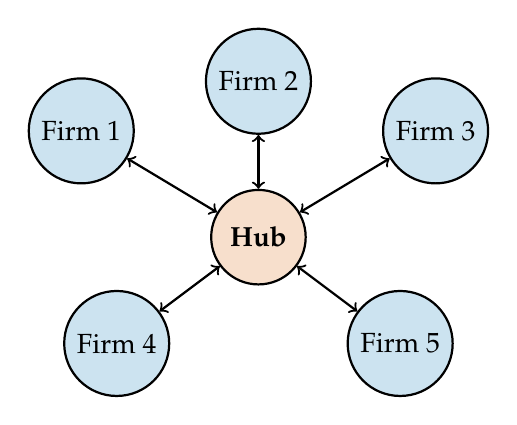
\begin{tikzpicture}[scale=0.9]
			% Hub
			\node[circle, draw, thick, fill=red!20, minimum size=1.2cm] (hub) at (0,0) {\textbf{Hub}};
			% Spokes
			\node[circle, draw, thick, fill=blue!20, minimum size=1cm] (s1) at (-2.5,1.5) {Firm 1};
			\node[circle, draw, thick, fill=blue!20, minimum size=1cm] (s2) at (0,2.2) {Firm 2};
			\node[circle, draw, thick, fill=blue!20, minimum size=1cm] (s3) at (2.5,1.5) {Firm 3};
			\node[circle, draw, thick, fill=blue!20, minimum size=1cm] (s4) at (-2,-1.5) {Firm 4};
			\node[circle, draw, thick, fill=blue!20, minimum size=1cm] (s5) at (2,-1.5) {Firm 5};
			% Connections
			\draw[thick, <->] (hub) -- (s1);
			\draw[thick, <->] (hub) -- (s2);
			\draw[thick, <->] (hub) -- (s3);
			\draw[thick, <->] (hub) -- (s4);
			\draw[thick, <->] (hub) -- (s5);
		\end{tikzpicture}
	\end{center}
	\vspace{3pt}
	\begin{wideitemize}
		\item \textbf{Legal issue:} Is hub liable? Are spokes colluding?
	\end{wideitemize}
\end{frame}

\begin{frame}{Multi-market contact}
	\begin{wideitemize}
		\item \textbf{Multi-market contact:} Same firms compete in multiple markets
		\item \textbf{Effect on collusion:}
		\begin{wideitemize}
			\vspace{5pt}
			\item More opportunities to punish deviators
			\item Deviation in market A triggers punishment in markets B, C, ...
			\item Increases total punishment $\rightarrow$ lowers $\delta^*$
		\end{wideitemize}
		\item \textbf{Example:} Airlines compete on multiple routes
		\begin{wideitemize}
			\vspace{5pt}
			\item American and United both fly NYC-LA and NYC-Chicago
			\item Price war on one route can spread to others
		\end{wideitemize}
		\item \textbf{Bernheim \& Whinston (1990):} Formalized this theory
	\end{wideitemize}
\end{frame}

\begin{frame}{Price wars and demand uncertainty}
	\begin{wideitemize}
		\item \textbf{Problem:} Firms can't observe rivals' prices directly
		\item Low demand could be:
		\begin{wideitemize}
			\vspace{5pt}
			\item Bad luck (demand shock)
			\item Or a rival secretly cutting prices
		\end{wideitemize}
		\item \textbf{Green \& Porter (1984):} Price wars as equilibrium
		\begin{wideitemize}
			\vspace{5pt}
			\item When demand is low, trigger ``punishment phase''
			\item Not because anyone cheated---just to maintain incentives
			\item Punishment is temporary (return to collusion after $T$ periods)
		\end{wideitemize}
		\item \textbf{Implication:} Price wars can occur without anyone deviating
		\item This explains why we see cyclical pricing in some industries
	\end{wideitemize}
\end{frame}

%%%%%%%%%%%%%%%%%%%%%%%%%%%%%%%%%%%%%%%%%%%%%%%%%%%%%%%%%%%%%
% DETECTION AND POLICY
%%%%%%%%%%%%%%%%%%%%%%%%%%%%%%%%%%%%%%%%%%%%%%%%%%%%%%%%%%%%%

\begin{frame}{Plan}
  \begin{wideenumerate}
    \item Collusion theory
    \item \textbf{Detection and policy}
  \end{wideenumerate}
\end{frame}

\begin{frame}{Detection probability and fines}
	\begin{wideitemize}
		\item In reality: cartels may be detected and punished
		\item \textbf{Each period:}
		\begin{wideitemize}
			\vspace{5pt}
			\item Detection probability: $\rho$
			\item Fine if detected: $F$
		\end{wideitemize}
		\item \textbf{Modified collusion condition:}
		\begin{align*}
			\delta^* = \frac{\pi^D - \pi^C + \rho F}{\pi^D - \pi^{NE} + \rho F}
		\end{align*}
		\item Higher $\rho$ or higher $F$ $\rightarrow$ higher $\delta^*$ $\rightarrow$ harder to collude
	\end{wideitemize}
\end{frame}

\begin{frame}{Worked example: Detection and fines}
	\begin{wideitemize}
		\item \textbf{Question:}
		\item Cartel earns $\pi^C = 100$ per period
		\item $\pi^{NE} = 25$, $\pi^D = 150$
		\item Detection probability $\rho = 0.1$, fine $F = 500$
		\item Find the minimum $\delta$ for collusion.
	\end{wideitemize}
	\vspace{10pt}
	\centering
	\textit{Take 3 minutes.}
\end{frame}

\begin{frame}{Worked example: Detection (solution)}
	\begin{solutionbox}[Solution]
		\begin{wideitemize}
			\item Expected fine per period: $\rho F = 0.1 \times 500 = 50$
			\item Apply formula:
			\begin{align*}
				\delta^* = \frac{\pi^D - \pi^C + \rho F}{\pi^D - \pi^{NE} + \rho F} = \frac{150 - 100 + 50}{150 - 25 + 50} = \frac{100}{175} = 0.571
			\end{align*}
			\item \textbf{Compare to no detection:}
			\begin{align*}
				\delta^*_{\text{no detection}} = \frac{150 - 100}{150 - 25} = \frac{50}{125} = 0.4
			\end{align*}
			\item Detection and fines make collusion harder (0.4 $\rightarrow$ 0.57)
		\end{wideitemize}
	\end{solutionbox}
\end{frame}

\begin{frame}{Criminal vs civil penalties}
	\begin{wideitemize}
		\item \textbf{In the US, price-fixing is a felony}
		\item \textbf{Civil penalties:}
		\begin{wideitemize}
			\vspace{5pt}
			\item Corporate fines (up to 10\% of affected commerce)
			\item Treble damages in private lawsuits
		\end{wideitemize}
		\item \textbf{Criminal penalties:}
		\begin{wideitemize}
			\vspace{5pt}
			\item Individual prison sentences (up to 10 years)
			\item Individual fines (up to \$1 million)
		\end{wideitemize}
		\item \textbf{Why criminal penalties matter:}
		\begin{wideitemize}
			\vspace{5pt}
			\item Executives can't pass prison time to shareholders
			\item Creates personal incentive not to collude
			\item Lysine: executives actually went to prison
		\end{wideitemize}
	\end{wideitemize}
\end{frame}

\begin{frame}{Optimal deterrence: Becker (1968)}
	\begin{wideitemize}
		\item \textbf{Expected cost of crime:} $\rho \times F$
		\item To deter, need: Expected cost $>$ Expected gain
		\item \textbf{Question:} How should we set $\rho$ and $F$?
		\item \textbf{Becker's insight:}
		\begin{wideitemize}
			\vspace{5pt}
			\item Detection is costly (investigations, lawyers)
			\item Fines are cheap to impose
			\item $\rightarrow$ Set $F$ very high, $\rho$ low
		\end{wideitemize}
		\item \textbf{Problem:} Firms may not have enough to pay huge fines
		\item \textbf{Solution:} Criminal penalties fill the ``gap''
	\end{wideitemize}
\end{frame}

\begin{frame}{Leniency programs}
	\begin{wideitemize}
		\item \textbf{Leniency:} First firm to report cartel gets reduced/zero fine
		\item \textbf{US Corporate Leniency Program (1993):}
		\begin{wideitemize}
			\vspace{5pt}
			\item First to report: automatic immunity
			\item Second: significant reduction possible
		\end{wideitemize}
		\item \textbf{Effect on incentives:}
		\begin{wideitemize}
			\vspace{5pt}
			\item Creates ``race to report''
			\item Each firm fears others will report first
			\item Destabilizes existing cartels
		\end{wideitemize}
	\end{wideitemize}
\end{frame}

\begin{frame}{Why leniency works}
	\begin{wideitemize}
		\item \textbf{Without leniency:}
		\begin{wideitemize}
			\vspace{5pt}
			\item If detected, everyone pays fine
			\item No incentive to report
		\end{wideitemize}
		\item \textbf{With leniency:}
		\begin{wideitemize}
			\vspace{5pt}
			\item First to report gets immunity
			\item Creates Prisoner's Dilemma within cartel
			\item Each firm thinks: ``Better report before they do''
		\end{wideitemize}
		\item \textbf{Result:} Cartel detection increased dramatically after 1993
		\item \textbf{Exam question:} ``Explain why leniency programs help detect cartels.''
	\end{wideitemize}
\end{frame}

\begin{frame}{Factors facilitating collusion}
	\begin{wideenumerate}
		\item \textbf{Few firms:} Easier to coordinate and monitor
		\item \textbf{Frequent interaction:} Higher effective $\delta$
		\item \textbf{Similar costs:} Easier to agree on price
		\item \textbf{Stable demand:} Easier to detect deviations
		\item \textbf{Homogeneous products:} Easier to monitor prices
		\item \textbf{Industry associations:} Facilitate communication
	\end{wideenumerate}
\end{frame}

\begin{frame}{Bid-rigging in auctions}
	\begin{wideitemize}
		\item \textbf{Bid-rigging:} Collusion in procurement auctions
		\item \textbf{Common schemes:}
		\begin{wideitemize}
			\vspace{5pt}
			\item \textbf{Bid rotation:} Firms take turns ``winning''
			\item \textbf{Bid suppression:} Some firms don't bid at all
			\item \textbf{Complementary bidding:} Losers submit high ``cover'' bids
			\item \textbf{Subcontracting:} Winner pays off losers
		\end{wideitemize}
		\item \textbf{Example:} Construction bid-rigging in NYC (1980s)
		\item Often easier to detect than retail price-fixing (paper trail)
	\end{wideitemize}
\end{frame}

\begin{frame}{T/F: Detection and policy}
	\textbf{True, False, or Not Enough Information?}
	\vspace{10pt}
	\begin{wideenumerate}
		\item Leniency programs reduce the total number of cartels that form.
		\item If detection probability doubles, collusion becomes twice as hard.
		\item Criminal penalties are more effective than fines because they can't be passed to shareholders.
		\item Tacit collusion is legal because firms don't explicitly communicate.
	\end{wideenumerate}
	\vspace{10pt}
	\centering
	\textit{Take 3 minutes.}
\end{frame}

\begin{frame}{T/F: Detection and policy (solutions)}
	\begin{solutionbox}[Solutions]
		\begin{wideenumerate}
			\item \textbf{NEI.} Leniency destabilizes existing cartels but may reduce fear of detection, potentially encouraging cartel formation. Empirically ambiguous.
			\item \textbf{FALSE.} From formula, $\rho$ appears in both numerator and denominator---effect is not linear.
			\item \textbf{TRUE.} Prison time is ``non-transferable''---executives face personal consequences.
			\item \textbf{TRUE.} (Generally) Without evidence of explicit agreement, parallel pricing is hard to prosecute.
		\end{wideenumerate}
	\end{solutionbox}
\end{frame}

\begin{frame}{Famous cartel cases}
	\begin{wideitemize}
		\item \textbf{Lysine cartel (1990s):}
		\begin{wideitemize}
			\vspace{5pt}
			\item Price-fixing among feed additive producers
			\item FBI surveillance, recorded meetings
		\end{wideitemize}
		\item \textbf{LCD screen cartel (2000s):}
		\begin{wideitemize}
			\vspace{5pt}
			\item Samsung, LG, Sharp, others
			\item \$1.4 billion in fines
		\end{wideitemize}
		\item \textbf{LIBOR scandal (2012):}
		\begin{wideitemize}
			\vspace{5pt}
			\item Banks manipulated interest rate benchmark
			\item \$9 billion in fines
		\end{wideitemize}
	\end{wideitemize}
\end{frame}

\begin{frame}{Detecting collusion: what regulators look for}
	\begin{wideitemize}
		\item \textbf{Pricing patterns:}
		\begin{wideitemize}
			\vspace{5pt}
			\item Parallel price changes
			\item Price rigidity despite cost changes
			\item Similar prices despite different costs
		\end{wideitemize}
		\item \textbf{Market characteristics:}
		\begin{wideitemize}
			\vspace{5pt}
			\item High concentration
			\item Frequent meetings/communication
			\item History of antitrust violations
		\end{wideitemize}
		\item \textbf{Whistleblowers:} Leniency program tips
	\end{wideitemize}
\end{frame}

\begin{frame}{Plus-factors in antitrust law}
	\begin{wideitemize}
		\item \textbf{Problem:} Parallel pricing is not illegal by itself
		\item \textbf{Courts require ``plus-factors'':} Evidence beyond parallel conduct
		\item \textbf{Common plus-factors:}
		\begin{wideitemize}
			\vspace{5pt}
			\item Actions against individual self-interest
			\item Secret meetings or communications
			\item Artificial standardization of products
			\item Exchange of price information
			\item Price increases during demand slumps
		\end{wideitemize}
		\item \textbf{Economic testimony:} Experts analyze whether behavior is consistent with competition
	\end{wideitemize}
\end{frame}

\begin{frame}{Algorithmic collusion: a new frontier}
	\begin{wideitemize}
		\item \textbf{Question:} Can algorithms collude without human instruction?
		\item \textbf{How it might work:}
		\begin{wideitemize}
			\vspace{5pt}
			\item Firms use pricing algorithms (AI/ML)
			\item Algorithms learn to ``cooperate'' through repeated interaction
			\item No explicit programming to collude
		\end{wideitemize}
		\item \textbf{Legal challenge:}
		\begin{wideitemize}
			\vspace{5pt}
			\item Traditional antitrust requires ``agreement''
			\item If algorithms learn collusion independently, is there agreement?
		\end{wideitemize}
		\item \textbf{Active research area:} Assad et al. (2024) on German retail gasoline
		\item Policy is still catching up
	\end{wideitemize}
\end{frame}

\begin{frame}{Collusion summary table}
	\begin{center}
		\small
		\begin{tabular}{|p{3.5cm}|p{4cm}|p{4cm}|}
			\hline
			\textbf{Concept} & \textbf{Key Formula/Idea} & \textbf{Policy Implication} \\
			\hline
			Critical discount factor & $\delta^* = \frac{\pi^D - \pi^C}{\pi^D - \pi^{NE}}$ & Lower $\delta^*$ = easier collusion \\
			\hline
			Detection \& fines & Increase $\rho F$ in formula & Higher penalties deter \\
			\hline
			Leniency & First to report = immunity & Creates ``race to confess'' \\
			\hline
			Multi-market contact & More markets = more punishment & Monitor multi-market firms \\
			\hline
			Plus-factors & Evidence beyond parallel pricing & Required for prosecution \\
			\hline
		\end{tabular}
	\end{center}
\end{frame}

\begin{frame}{Course connection: collusion and mergers}
	\begin{wideitemize}
		\item \textbf{Merger review considers coordinated effects:}
		\begin{wideitemize}
			\vspace{5pt}
			\item Will the merger make collusion easier?
			\item Fewer firms $\rightarrow$ lower $\delta^*$ $\rightarrow$ easier collusion
		\end{wideitemize}
		\item \textbf{What makes post-merger collusion more likely?}
		\begin{wideitemize}
			\vspace{5pt}
			\item Merger creates symmetric cost structures
			\item Merger eliminates a ``maverick'' (aggressive competitor)
			\item Merger increases multi-market contact
		\end{wideitemize}
		\item \textbf{HW2 connection:} Your merger simulation focuses on unilateral effects, but DOJ also considers coordinated effects
	\end{wideitemize}
\end{frame}

%%%%%%%%%%%%%%%%%%%%%%%%%%%%%%%%%%%%%%%%%%%%%%%%%%%%%%%%%%%%%
% KEY POINTS
%%%%%%%%%%%%%%%%%%%%%%%%%%%%%%%%%%%%%%%%%%%%%%%%%%%%%%%%%%%%%

\begin{frame}{Key Points}
	\vspace{11pt}
	\begin{wideenumerate}
		\item \textbf{Critical discount factor:} $\delta^* = \frac{\pi^D - \pi^C}{\pi^D - \pi^{NE}}$
		\item \textbf{Cournot with N firms:} $\delta^* = \frac{(N+1)^2}{N^2 + (N+1)^2}$
		\item \textbf{Bertrand with N firms:} $\delta^* = \frac{N-1}{N}$
		\item More firms $\rightarrow$ generally harder to collude
		\item \textbf{Detection and fines} raise $\delta^*$: $\delta^* = \frac{\pi^D - \pi^C + \rho F}{\pi^D - \pi^{NE} + \rho F}$
		\item \textbf{Leniency programs:} Create ``race to report,'' destabilize cartels
		\item Collusion easier with: few firms, frequent interaction, similar costs
	\end{wideenumerate}
\end{frame}

\begin{frame}{Next time}
	\begin{wideitemize}
		\item \textbf{Lecture 13:} Final Review
		\begin{wideitemize}
			\vspace{5pt}
			\item Comprehensive review of Part 1 and Part 2
			\item Practice problems for final exam
		\end{wideitemize}
		\item \textbf{HW2 due before Lecture 13}
	\end{wideitemize}
\end{frame}

\end{document}
